% !TEX root = ../thesis.tex

\chapter{Analytical part}\label{sec:analytical}

Linear prediction is~a statistical method used to predict future values based on historical data.
The Durbin-Levinson algorithm is a~method for solving the~linear prediction problem for autoregressive (AR)
models\footnote{Autoregressive (AR) models are time series models that describe the~the~relationship between the~current
value of a~variable and its past values. In~an~autoregressive model, each observation is modeled as a~linear
combination of past observations, with weights called AR coefficients. AR models are widely used in various fields
such as economics, engineering, and finance for modeling and forecasting time series data. the~order of the~AR model, denoted as "p", refers to the~number of past values used to predict the~current value. For example,~an~AR(1) model uses
only the~previous observation to predict the~current value, while~an~AR(2) model uses the~previous two observations.},
which are models where the~current output depends on previous outputs. the~algorithm solves the~linear prediction
problem by finding the~coefficients of the~AR model that minimize the~prediction error. the~resulting AR coefficients
can be used to make predictions about future values based on past observations. This method should be used with
using the~pattern of linear relationship between the~independent and dependent variables.
Here's a~basic outline of the~steps involved in using linear prediction to forecast sales data:\\
\begin{enumerate}
    \item Collect sales data: Gather the~historical sales data for the~product or service that we want to forecast.
    \item Plot the~data: Plot the~sales data over time to visually inspect the~trend and identify any patterns.
    \item Choose a~model: Select~an~appropriate linear model to represent the~relationship between the~independent and
    dependent variables in the~data. For example, we might choose a~simple linear regression model.
    \item Train the~model: Train the~selected model on the~historical sales data using a~method such as least squares
    regression.
    \item Make predictions: Use the~trained model to make predictions on future sales data. We may want to generate
    predictions for several months or years in advance.
    \item Evaluate the~model: Assess the~accuracy of the~predictions by comparing them to the~actual sales data.
    Use metrics such as mean absolute error or root mean squared error to quantify the~model's performance.
    \item Refine the~model: If necessary, refine the~model by adding additional independent variables or
    transforming the~existing variables. Repeat the~training and evaluation steps until we have a~model that
    provides accurate forecasts.
\end{enumerate}
For shift calculation in longterm prediction can be used autocorrelation method, in this thesis neural network for
identification shift will be developed and similar mechanism for optimal order detection.

\section{Models used for sales data forecasting}\label{sec:models}
There are several mathematical models used for sales prediction, including Time series models~\ref{sec:timeseries} which are used to analyze and forecast sales data over time, such as seasonal patterns, trends, and fluctuations. Regression models~\ref{sec:regression} to use historical data to determine the~relationship between sales and one or more independent variables, such as price, promotion, and advertising. Decision tree models~\ref{sec:trees} use a~tree-like structure to make decisions based on the~relationship between sales and multiple independent variables and machine learning models~\ref{sec:ml} to use algorithms such as neural networks and support vector machines to make predictions based on patterns in the~data. \\
\\
The choice of mathematical model depends on the~characteristics of the~data, the~desired level of accuracy, and the
computational resources available.
\\

\subsection{Time-series models}\label{sec:timeseries}
Time-series models are mathematical models used to analyze and forecast data that are collected over time~\cite{Cryer}.
These models are used to study and make predictions about the~trends, patterns, and behavior of the~data over time,
taking into account historical values and their relationship with the~present. Time-series models are widely
used in areas such as economics, finance, and weather forecasting, among others. the~models are based on various
statistical techniques, including ARIMA (AutoRegressive Integrated Moving Average), SARIMA (Seasonal ARIMA),
and exponential smoothing, among others. the~goal of time-series modeling is to build a~mathematical representation
of the~underlying process that generates the~time-series data, allowing for accurate prediction of future values.
Time-series models are statistical models used to analyze and make predictions about time-dependent data. They are
widely used in various fields, including finance, economics, engineering, and social sciences.
\\
Time-series models make use of past values of a~variable to predict future values.
They assume that there is a~pattern or trend in the~data that can be used to forecast future behavior.
Some commonly used time-series models include:
\begin{itemize}
    \item Autoregressive Integrated Moving Average (ARIMA). This model is used to analyze and forecast stationary
    time-series data. It consists of three components: autoregression, differencing, and moving average.
    \item Seasonal Autoregressive Integrated Moving Average (SARIMA) is~an~extension of ARIMA
    that takes into account seasonal patterns in the~data.
    \item Exponential Smoothing (ETS) is used to forecast time-series data that has a~trend
    and/or seasonality. It uses a~smoothing parameter to assign more or less weight to past observations
    based on their recency.
    \item Vector Autoregression (VAR) is used when there are multiple time-series variables
    that influence each other. It can be used to analyze the~relationships between these variables and to make
    predictions about their future be   havior.
    \item These models are valuable tools for analyzing and predicting time-series data, but they require careful
    consideration of the~specific characteristics of the~data being analyzed and the~appropriate model to use.
\end{itemize}

\subsection{Regression models}\label{sec:regression}
Regression models are a~type of statistical models used to examine the~relationship between a~dependent variable
and one or more independent variables~\cite{Fahrmeir}.
The goal of regression analysis is to model the~relationship between these variables and make predictions about
the dependent variable based on the~values of the~independent variables. Regression models are widely used in many
fields, including economics, finance, marketing, and social sciences, to make predictions and understand the
relationship between variables. There are several types of regression models, including:
\begin{itemize}
    \item Linear regression is a~simple regression model where the~relationship between the~dependent and independent
    variables is modeled using a~linear equation.
    \item Logistic regression is used for binary classification problems where the~dependent variable is binary and the~goal is to model the~relationship between the~independent variables and the~probability of the~dependent
    variable being either 0 or 1.
    \item Multiple regression is used when there are multiple independent variables and the~goal is to model the
    relationship between all of these variables and the~dependent variable.
    \item Polynomial regression is used when the~relationship between the~dependent and independent variables
    is non-linear and can be modeled using a~polynomial equation.
\end{itemize}

The choice of regression model depends on the~nature of the~data and the~research question being asked.

\subsection{Decision tree models}\label{sec:trees}
Decision tree models are a~type of machine learning models used for both regression and classification
tasks~\cite{Kotsiantis}. They are tree-like structures that make predictions by breaking down a~dataset into
smaller and smaller subsets, based on the~values of the~input variables. At each internal node of the~tree,
a decision rule is used to split the~data based on the~value of a~feature, and the~process continues until the
data are separated into homogeneous groups, or leaves.
The predictions are then made based on the~average or majority class in each leaf node. On figure~\ref{fig:example_tree} we can see example schema how the~decision tree works.\\
\begin{figure}
    \centering
    \begin{tikzpicture}
        \Tree [.S        [.NP            [.Det the ]
                [.N cat ]
            ]
            [.VP            [.V chased ]
                [.NP                [.Det the ]
                    [.N mouse ]
                ]
            ]
        ]
    \end{tikzpicture}   
    \caption{Example of decission tree flow.}\label{fig:example_tree}
\end{figure}
\\
Decision trees have several advantages, including ease of interpretability, handling of non-linear relationships,
and ability to handle both categorical and numerical data. Some examples of decision tree algorithms are CART
(Classification and Regression Tree) and Random Forest.
\\
The decision tree model is trained using a~dataset, and the~tree structure is built using a~greedy algorithm
that seeks to maximize the~reduction in impurity of the~target variable at each split. the~model can then be used
to make predictions on new data by following the~decision rules in the~tree.
\subsection{Machine learning models}\label{sec:ml}
Machine learning models are a~subset of artificial intelligence that allows computers to learn and make
predictions or decisions without being explicitly programmed. Machine learning models are based on algorithms
that use statistical methods to find patterns in data and make predictions about new, unseen data.
\\
There are several types of machine learning models, including \textbf{Supervised learning} where the~model is trained on labeled data, with the~goal of learning the~relationship between the~input features and the~target variable, and making predictions about the~target variable for new, unseen data.
\textbf{Unsupervised learning} where the~model is trained on unlabeled data, with the~goal of finding patterns or structure in the~data, such as clustering or dimensionality reduction. \textbf{Reinforcement learning} where the~model learns by receiving rewards or penalties for its actions in~an~environment, with the~goal of maximizing the~reward over time. \textbf{Deep learning} a~subset of machine learning that uses artificial neural networks with multiple hidden layers to model complex relationships in the~data. 

The choice of machine learning model depends on the~problem being solved and the~type of data being used. Machine
learning models have been applied to a~wide range of tasks, including image and speech recognition, natural language
processing, and predictive modeling. Advances in machine learning (ML), faster processors and the~availability of
digitized healthcare data have contributed to a~growing number of papers describing ML applications in healthcare~\cite{Chen}.\\
\newpage
\noindent \textbf{K-Nearest Neighbors (KNN)} \label{sec:knn}\\
Machine learning algorithms, K-Nearest Neighbors (KNN), is a~type of artificial intelligence that allows
computers to learn and make decisions based on data. KNN is a~simple yet effective algorithm used for
classification and regression tasks in supervised learning.\\
\\
KNN is a~non-parametric algorithm, which means it doesn't make any assumptions about the~underlying
distribution of the~data. Instead, it uses the~similarity between data points to classify or predict the~target
variable. the~algorithm works by finding the~k-nearest neighbors to a~new data point and then assigning the~class
label of the~majority of those neighbors to the~new data point.\\
\\
For example, if we have a~dataset of images with labels indicating whether each image contains a~cat or a~dog,
we can use KNN to classify a~new image by finding the~k-nearest neighbors to the~new image and assigning the
label of the~majority of those neighbors to the~new image.\\
\\
KNN is a~relatively simple algorithm, but it can be very effective when applied to the~right problems.
It is particularly useful in cases where the~decision boundary is nonlinear or where there is no clear
separation between classes. However, KNN can be computationally expensive when working with large datasets, and
it may not perform well in high-dimensional spaces.


\section{Neural networks} \label{sec:nn}
A neural network is a~type of machine learning algorithm inspired by the~structure and function of biological neurons
in the~human brain. It is composed of interconnected nodes, called neurons, that are organized into layers. the~input
layer receives raw data, such as images or text, and passes it on to the~hidden layers, which perform calculations and
apply weights to the~input data to create a~prediction. Finally, the~output layer produces the~final prediction
or classification.\\
\\
As we can see on image \ref{fig:perceptron} each input $X_n$ should be properly weighted by a~certain weight $W_n$ before
all the~signals enter the~summation stage. Afterwards, the~weighted summation is forwarded into the~activation unit
producing the~neuron’s output signal.
\begin{center}
    \begin{figure}[!ht]
        \centering
        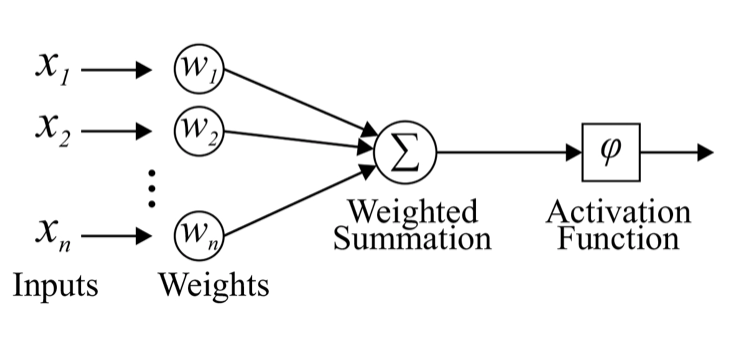
\includegraphics[width=1\textwidth]{figures/nn}
        \caption{Perceptron preview. \cite{Mourgias-Alexandris:19}}
        \label{fig:perceptron}
    \end{figure}
\end{center}
Neural networks are trained on large datasets using a~process called backpropagation, which adjusts the~weights and
biases of the~neurons to minimize the~error between the~predicted output and the~actual output. Once a~neural network
has been trained, it can be used to make predictions on new data.\\
\\
A neuron is a~basic building block of a~neural network, also known as~an~artificial neuron or a~perceptron.
It is modeled after the~biological neuron in the~human brain, which receives input signals from other neurons,
processes them, and sends output signals to other neurons.\\
\\
In a~neural network, a~neuron receives input from other neurons or directly from the~input data, applies a~mathematical
function to the~input, and produces~an~output that is sent to other neurons in the~network. the~input to a~neuron is
usually a~vector of numbers, and each input is multiplied by a~corresponding weight. the~neuron then sums up the
weighted inputs, adds a~bias term, and applies~an~activation function to the~result.\\
\\
The purpose of the~activation function is to introduce nonlinearity into the~neuron, which allows the~neural network
to learn complex patterns and relationships in the~data. There are several different types of activation functions
that can be used, such as the~sigmoid function, ReLU (Rectified Linear Unit) function, and tanh (hyperbolic tangent)
function.\\
\\
The output of a~neuron is typically fed into other neurons in the~next layer of the~neural network. the~weights and
biases of the~neurons are adjusted during the~training process using a~technique called backpropagation, which involves
computing the~gradient of the~error with respect to the~weights and updating them using~an~optimization algorithm such
as stochastic gradient descent.\\
Overall, the~neurons in a~neural network work together to learn patterns and relationships in the~input data and produce
output that can be used for a~variety of tasks, such as classification, regression, and prediction.\\
Neural networks have been successfully applied in a~wide range of fields, including image and speech recognition, natural language processing, and autonomous vehicles, among others.
Neural networks can be broadly classified into the~following types:\\
\\
\textbf{Feedforward Neural Networks}\\
These are the~most basic type of neural networks, where the~information flows
only in one direction,from input to output. These networks can have one or more hidden layers and are often used for classification or regression tasks. Shema on basic feedforward NN is on fig~\ref{fig:ff}
    \begin{center}
        \begin{figure}[!ht]
            \centering
            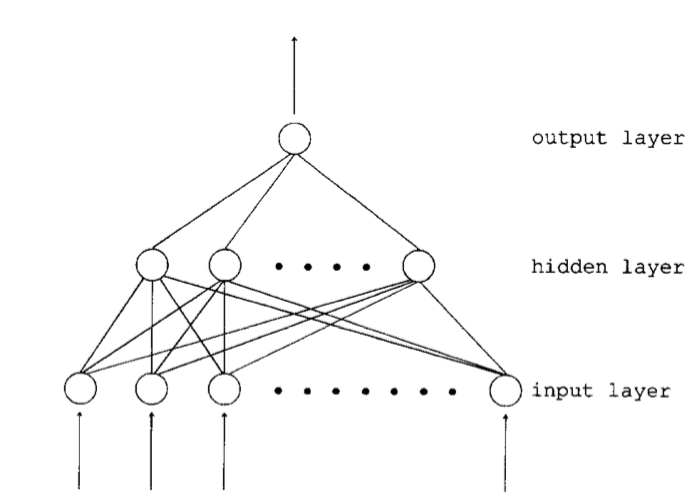
\includegraphics[width=0.6\textwidth]{figures/ff}
            \caption{Typical feed-forward neural network composed of three layers. \cite{svozil1997quantum}}
            \label{fig:ff}
        \end{figure}
    \end{center}
\textbf{Convolutional Neural Networks (CNNs)}\\
These networks are specialized for processing images and are commonly used in computer vision tasks. They use convolutional layers to extract features from images and can learn to recognize patterns and objects in images see in fig~\ref{fig:cn}
    \begin{center}
        \begin{figure}[!ht]
            \centering
            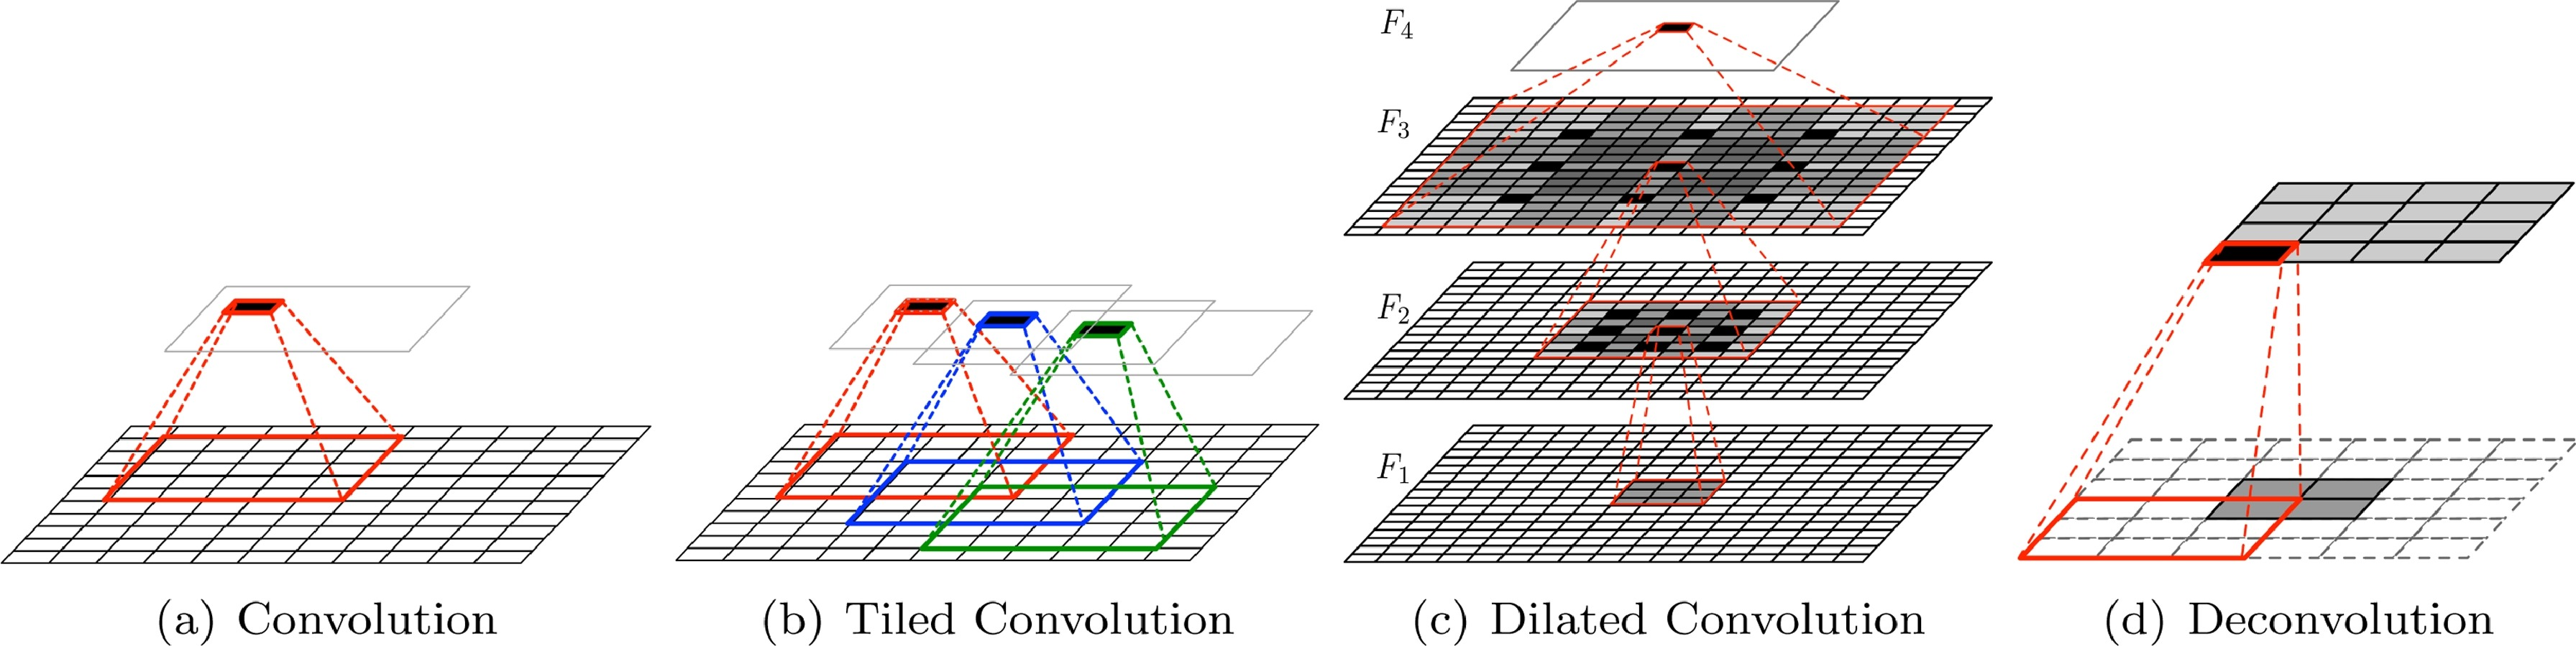
\includegraphics[width=0.8\textwidth]{figures/cn}
            \caption{Illustration of (a) Convolution, (b) Tiled Convolution, (c) Dilated Convolution, and (d)
                Deconvolution. \cite{GU2018354}}
            \label{fig:cn}
        \end{figure}
    \end{center}
\textbf{Recurrent Neural Networks (RNNs)}\\
These networks are designed to work with sequential data, such as time-series or natural language data. They have loops that allow information to be passed from one time-step to the~next, enabling them to capture temporal dependencies in the~data, described on fig~\ref{fig:rn}
    \begin{center}
        \begin{figure}[!ht]
            \centering
            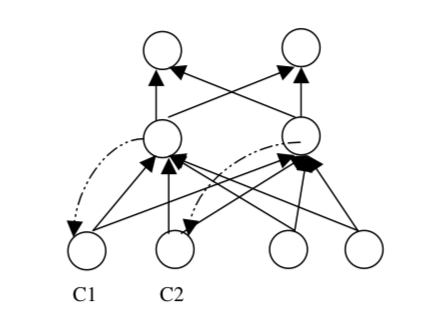
\includegraphics[width=0.8\textwidth]{figures/rn}
            \caption{Typical recurrent network. \cite{medsker2001recurrent}}
            \label{fig:rn}
        \end{figure}
    \end{center}
\textbf{Long Short-Term Memory Networks (LSTMs)}\\
These are a~type of RNN that are designed to address the~problem of vanishing gradients in traditional RNNs. They use memory cells and gates to selectively retain or forget information over time, making them well-suited for learning from long sequences. As you can see on fig~\ref{fig:ltmn} color indicates degree of memory activation.
    \begin{center}
        \begin{figure}[!ht]
            \centering
            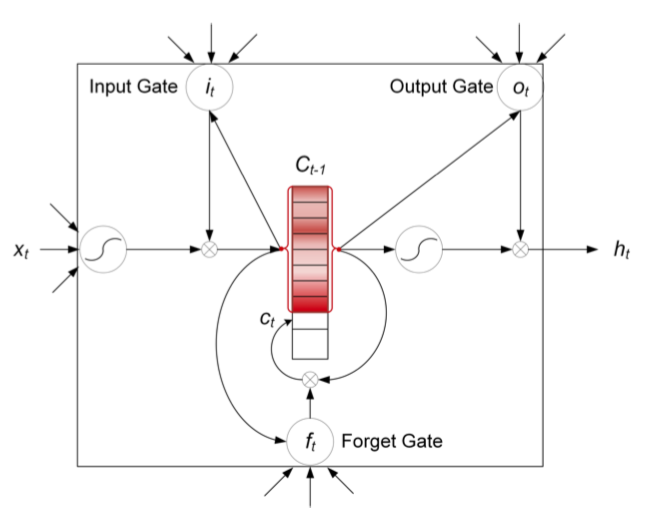
\includegraphics[width=0.4\textwidth]{figures/ltmn}
            \caption{Long short-term memory network. \cite{cheng2016long}}
            \label{fig:ltmn}
        \end{figure}
    \end{center}
\textbf{Autoencoder Neural Networks}\\
These networks are used for unsupervised learning and are designed to learn a~compressed representation of the~input data. As we can see on figure~\ref{fig:ann} they consist of~an~encoder that maps the~input data to a~compressed representation, and a~decoder that maps the~compressed representation back to the~original data.
    \begin{center}
        \begin{figure}[!ht]
            \centering
            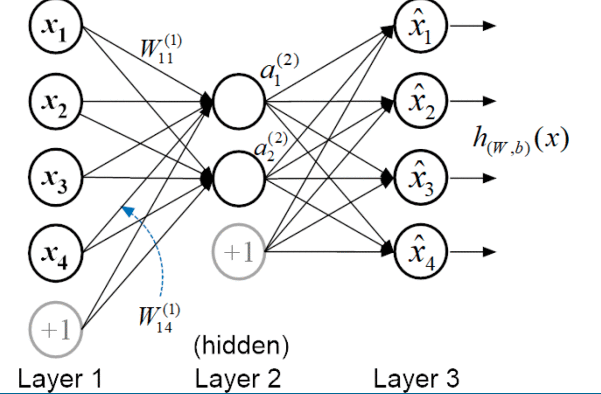
\includegraphics[width=0.5\textwidth]{figures/ann}
            \caption{An autoencoder neural network. \cite{luo2018distributed}}
            \label{fig:ann}
        \end{figure}
    \end{center}
\textbf{Generative Adversarial Networks (GANs)}\\
These networks consist of two networks, a~generator and a~discriminator (see on figure~\ref{fig:gan}), that are trained together in a~game-theoretic framework. the~generator is trained to generate realistic data samples, while the~discriminator is trained to distinguish between real and generated data samples.
    \begin{center}
        \begin{figure}[!ht]
            \centering
            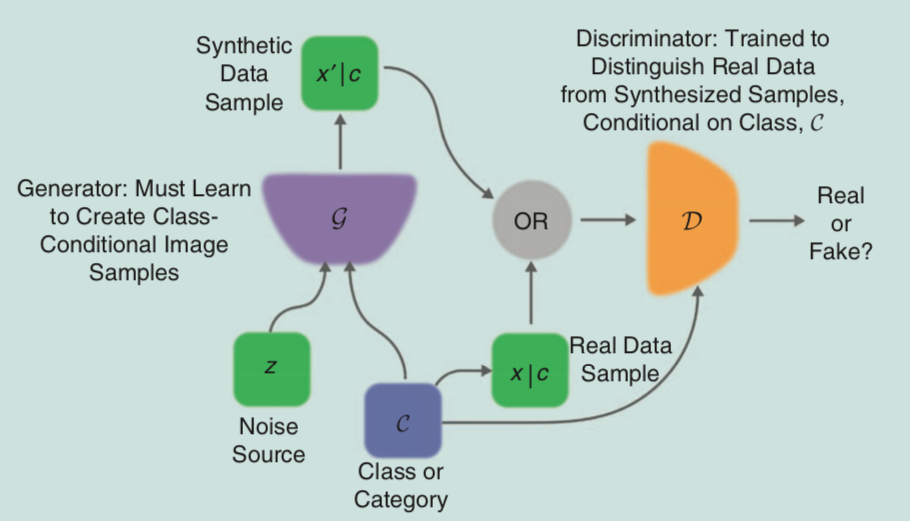
\includegraphics[width=0.5\textwidth]{figures/gan}
            \caption{The conditional GAN schema. \cite{creswell2018generative}}
            \label{fig:gan}
        \end{figure}
    \end{center}

These are some of the~most common types of neural networks, but there are many other specialized types of neural
networks that have been developed for specific tasks, such as object detection, speech recognition, and
natural language processing.\\

\subsection{Classification} \label{subsec:clasification}
Neural network data classification is a~technique for categorizing data into different classes or categories based on
patterns and features present in the~data. a~neural network is a~type of machine learning algorithm that is modeled
after the~structure and function of the~human brain. It is composed of interconnected nodes or neurons that are
organized into layers.\\
In a~classification task, the~neural network is trained on a~dataset that is labeled with the~correct
class for each example. During training, the~network learns to recognize patterns and features in the~input data
that are associated with each class. the~process of training involves adjusting the~weights and biases of the~neurons
in the~network to minimize the~error between the~predicted class and the~actual class of each example in the
training set.\\
Once the~neural network is trained, it can be used to classify new, unseen examples by inputting the~data into
the network and obtaining a~prediction of the~most likely class. the~output of the~neural network is a~probability
distribution over the~different classes, with the~highest probability indicating the~predicted class.\\
Neural network data classification has been successfully applied to a~wide range of tasks, including image
classification, speech recognition, natural language processing, and fraud detection, among others~\cite{feraud2002methodology}.

\subsection{Activation functions} \label{subsec:nnaf}
There are several types of activation functions~\cite{geron2022hands} used in neural networks, as we can see on figure~\ref{fig:activationfunctions} including:
\begin{itemize}
    \item Sigmoid Function: the~sigmoid function is a~commonly used activation function that maps any input value
    to a~value between 0 and 1. It is typically used in binary classification problems and in the~output layer of
    neural networks that produce probability estimates~\ref{fig:sigmoid}.
    \item ReLU (Rectified Linear Unit): the~ReLU function is another popular activation function that maps any
    input value less than 0 to 0, and any input value greater than or equal to 0 to the~input value itself.
    It is computationally efficient and has been shown to work well in deep neural networks~\ref{fig:relu}.
    \item Tanh Function: the~tanh (hyperbolic tangent) function is similar to the~sigmoid function,
    but it maps input values to a~range between -1 and 1. It is commonly used in the~hidden layers of neural networks~\ref{fig:tahn}.
    \item Softmax Function: the~softmax function is often used in the~output layer of neural networks that produce
    multi-class classification predictions. It maps the~outputs to a~probability distribution over the~possible classes~\ref{fig:sigmsoftmaxoid}.
    \item Leaky ReLU: the~Leaky ReLU function is similar to the~ReLU function, but it allows a~small, non-zero
    gradient when the~input value is negative. This can help to prevent the~"dying ReLU" problem, where some ReLU
    units become inactive and stop contributing to the~network's output~\ref{fig:leakyrelu}.
    \item ELU (Exponential Linear Unit): the~ELU function is similar to the~ReLU function, but it allows negative
    values to have non-zero outputs. This can help to prevent the~"dying ReLU" problem and can improve the
    performance of deep neural networks~\ref{fig:elu}.
\end{itemize}
These are some of the~most commonly used activation functions in neural networks, but there are many other types of
activation functions that have been developed for specific tasks or to address certain problems.

\begin{figure}
    \centering
    \begin{subfigure}[b]{0.4\textwidth}
        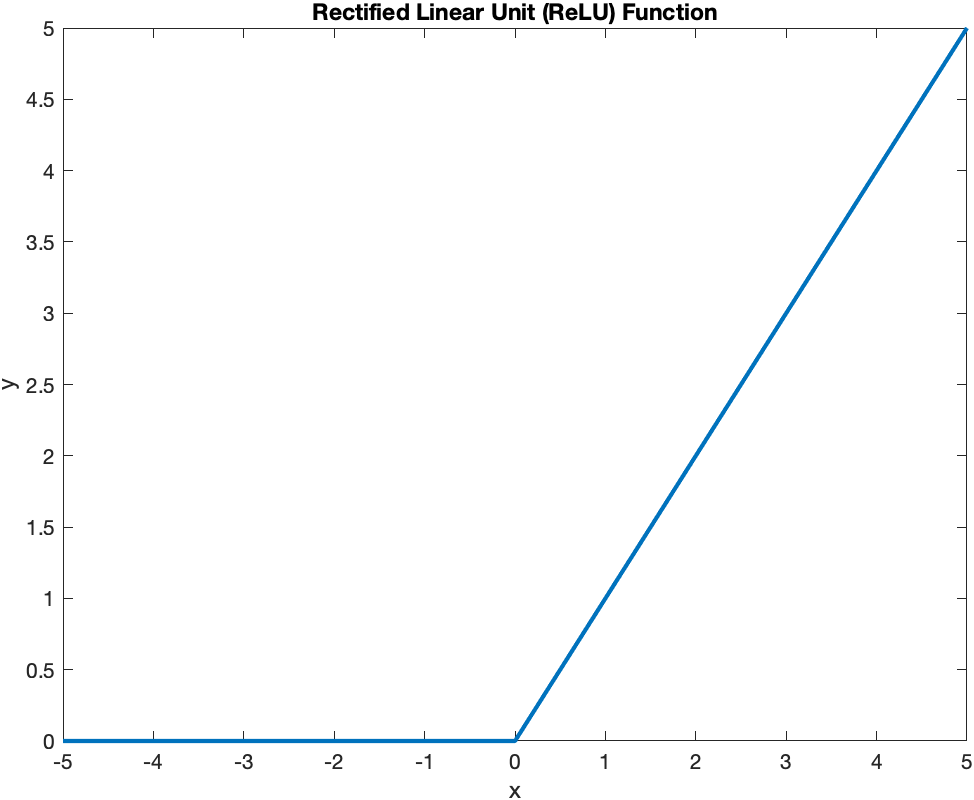
\includegraphics[width=\textwidth]{figures/relu}
        \caption{ReLU function}
        \label{fig:relu}
    \end{subfigure}
    \hspace{0.1\textwidth}
    \begin{subfigure}[b]{0.4\textwidth}
        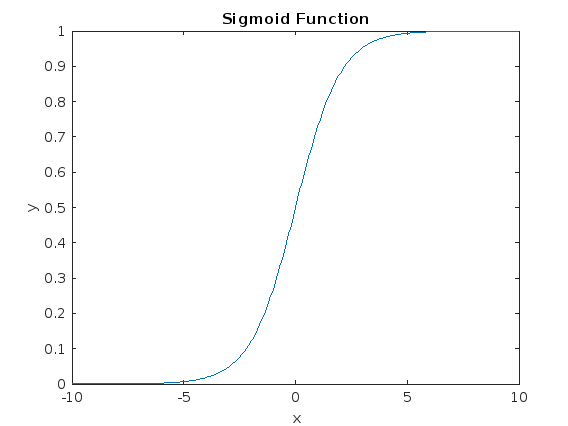
\includegraphics[width=\textwidth]{figures/sigmoid}
        \caption{Sigmoid function}
        \label{fig:sigmoid}
    \end{subfigure}
    \begin{subfigure}[b]{0.4\textwidth}
        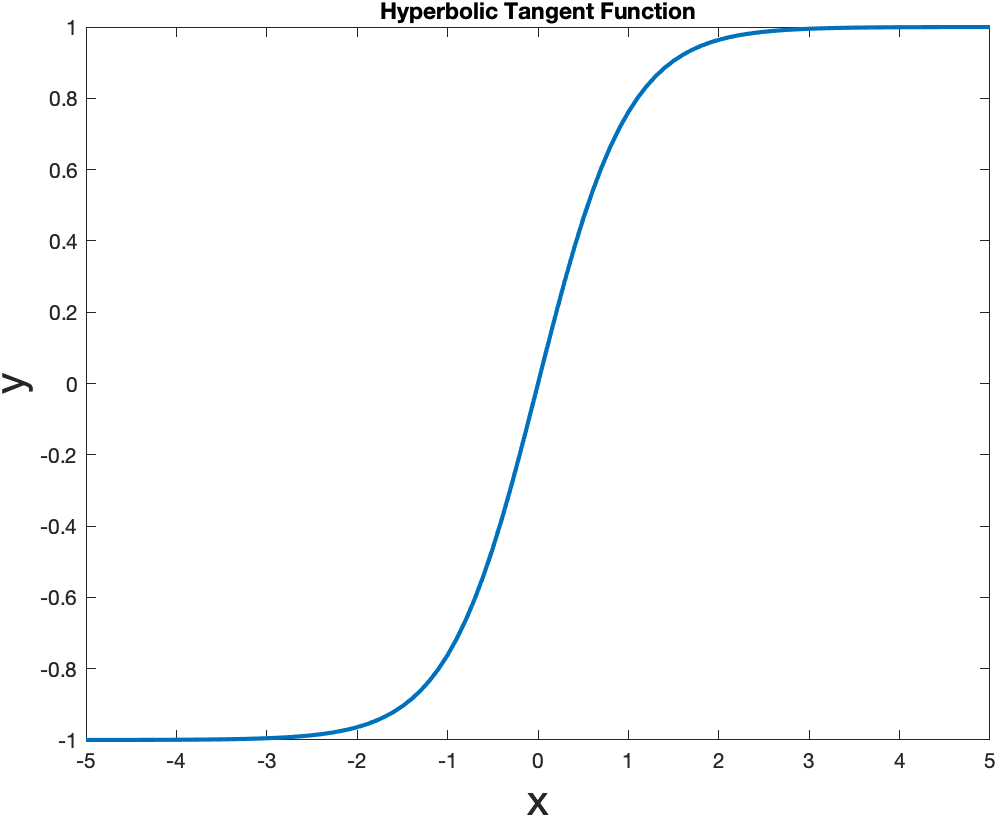
\includegraphics[width=\textwidth]{figures/tanh}
        \caption{Tanh function}
        \label{fig:tahn}
    \end{subfigure}
    \hspace{0.1\textwidth}
    \begin{subfigure}[b]{0.4\textwidth}
        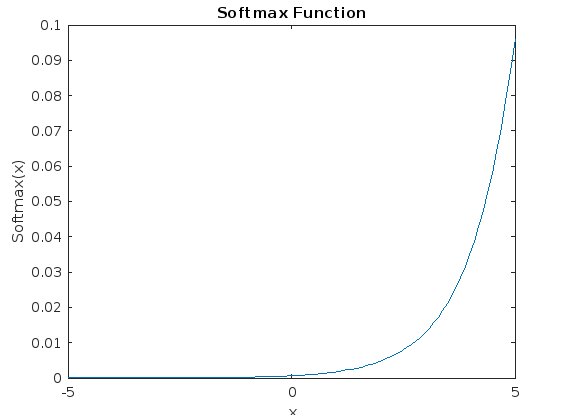
\includegraphics[width=\textwidth]{figures/softmax}
        \caption{Softmax function}
        \label{fig:sigmsoftmaxoid}
    \end{subfigure}
    \begin{subfigure}[b]{0.4\textwidth}
        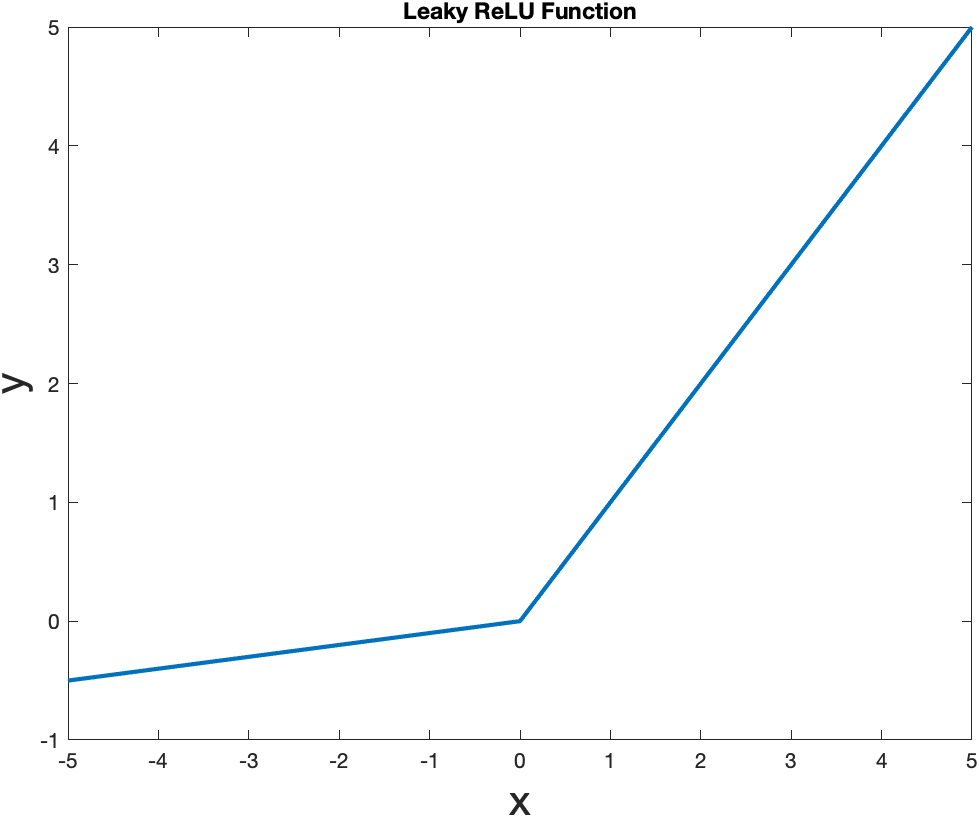
\includegraphics[width=\textwidth]{figures/leakyrelu}
        \caption{Leaky ReLU function}
        \label{fig:leakyrelu}
    \end{subfigure}
    \hspace{0.1\textwidth}
    \begin{subfigure}[b]{0.4\textwidth}
        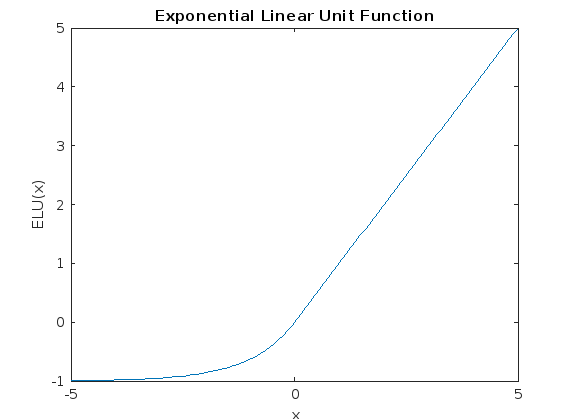
\includegraphics[width=\textwidth]{figures/elu}
        \caption{ELU function}
        \label{fig:elu}
    \end{subfigure}
    \caption{Neural network activation functions.}
    \label{fig:activationfunctions}
\end{figure}

\subsection{Application of neural netwrok in prediction} \label{subsec:nnprediction}
Neural networks can be used for long-term linear prediction in time-series data, including speech, health, and
stock data. Neural networks can be trained to model and forecast the~patterns in the~data, including shifts in
the long-term linear prediction. Neural networks have been shown to be effective in capturing the~complex relationships
between variables in time-series data, and can learn to identify subtle patterns and trends that may be difficult
to detect using traditional statistical methods. In the~context of long-term linear prediction, neural networks can be
trained on historical data to identify prev    atterns and trends in the~data and make predictions for future values.
They can also be used to detect shifts in the~long-term linear prediction, which can be useful for identifying
changes in the~underlying processes that generate the~data. However, it's important to note that neural networks
can be computationally expensive and require large amounts of data to train effectively. They also require careful
tuning of hyperparameters and selection of appropriate architecture to achieve good performance.
In addition, the~interpretation of the~results of a~neural network can be more challenging than with traditional
statistical methods. Overall, neural networks can be a~powerful tool for long-term linear prediction in time-series
data, including shifts in the~data, but their use should be carefully considered based on the~specific
application and available data.


\section{Linear prediction} \label{sec:lp}
Linear prediction is a~statistical technique used to forecast future values based on past observations. It is a~method
for modeling the~relationship between a~dependent variable and one or more independent variables in a~linear form.
The goal of linear prediction is to find the~best linear approximation of the~relationship between the~variables,
which can then be used to make predictions about future values of the~dependent variable.
\\
Linear prediction can be performed using simple linear regression or multiple linear regression, depending on the
number of independent variables involved~\cite{Parks}. In simple linear regression, a~single independent variable is
used to predict the~value of the~dependent variable, while in multiple linear regression, multiple independent
variables are used to make the~prediction.
\\
Linear prediction models are commonly used in finance, economics, and engineering, among other fields, to forecast
future values of time series data, such as stock prices, sales, or demand. the~accuracy of linear prediction models
depends on several factors, including the~quality of the~data, the~choice of independent variables, and the~degree of
linearity in the~relationship between the~variables.

\subsection{Short-term linear prediction} \label{subsec:shortlp}

Short-term linear prediction~\cite{Riahy} refers to the~use of linear prediction techniques to make predictions about
the near-term future values of a~time series. It is used to forecast future values of a~dependent variable based on
its past values and any relevant independent variables.
\\
In short-term linear prediction, the~focus is on accurately predicting the~next few values of the~dependent variable,
typically in the~range of several weeks to a~few months. the~linear prediction models used for short-term
forecasting are typically simple and straightforward, often using a~small number of independent variables.
The goal is to provide a~quick and easily interpretable forecast that can be used to make operational decisions in
the short-term.
Consider a~signal $x(n)$ that is modeled using a~linear predictor. the~linear predictor is defined as:

\begin{equation}
  \hat{x}(n) = \sum_{i=1}^{p} a_i x(n-i),
  \label{eq:linear-predictor}
\end{equation}

where $\hat{x}(n)$ is the~predicted value of $x(n)$, $p$ is the~order of the~predictor, and $a_i$ are the~predictor coefficients. the~predictor coefficients can be found by minimizing the~prediction error:

\begin{equation}
  e(n) = x(n) - \hat{x}(n),
  \label{eq:prediction-error}
\end{equation}

Using the~least squares method, we can find the~predictor coefficients by minimizing the~sum of squared prediction errors:

\begin{equation}
  \min_{a_1,\dots,a_p} \sum_{n=1}^{N} e^2(n),
  \label{eq:least-squares}
\end{equation}

This can be solved analytically using the~following matrix equation:

\begin{equation}
  \begin{bmatrix}
    r(0) & r(1) & \cdots & r(p-1) \\
    r(1) & r(0) & \cdots & r(p-2) \\
    \vdots & \vdots & \ddots & \vdots \\
    r(p-1) & r(p-2) & \cdots & r(0)
  \end{bmatrix}
  \begin{bmatrix}
    a_1 \\
    a_2 \\
    \vdots \\
    a_p
  \end{bmatrix}
  =
  \begin{bmatrix}
    r(1) \\
    r(2) \\
    \vdots \\
    r(p)
  \end{bmatrix},
  \label{eq:matrix-equation}
\end{equation}

where $r(k)$ is the~autocorrelation function of the~signal $x(n)$ defined as:

\begin{equation}
  r(k) = \frac{1}{N} \sum_{n=k+1}^{N} x(n) x(n-k),
  \label{eq:autocorrelation}
\end{equation}

Common techniques for short-term linear prediction include moving average models, exponential smoothing, and
autoregressive models. These methods use the~historical data of the~time series to model the~relationship between the
dependent and independent variables, and to make predictions about future values. the~accuracy of short-term linear
predictions can be evaluated using metrics such as mean absolute error, mean squared error, or the~correlation
coefficient between the~actual and predicted values.

\subsection{Long-term linear prediction}\label{subsec:longlp}
Long-term linear prediction is a~technique commonly used in the~analysis of time-series data, including health data.
In the~context of health data, the~shift of long-term linear prediction refers to the~way in which the~patterns in the
data change over time, reflecting changes in the~underlying health status of the~individual or population being studied.\\
For example, in the~case of a~patient with a~chronic disease, the~long-term linear prediction of their health data may
show a~gradual decline over time as the~disease progresses. Alternatively, the~data may show periodic shifts
corresponding to changes in medication or other interventions. In population health studies, long-term linear
prediction can be used to identify trends and patterns in health outcomes over time. For example, a~long-term linear
prediction model might be used to track changes in the~prevalence of a~particular disease or condition
over a~period of several years, taking into account factors such as demographic changes and changes in healthcare policy.
Overall, the~shift of long-term linear prediction for health data reflects the~dynamic nature of health status and
healthcare interventions, and can be a~powerful tool for understanding trends and patterns in health outcomes over time.
\\
Long-term linear prediction refers to the~use of linear prediction techniques to make predictions about the~future
values of a~time series over~an~extended period of time, typically several months to several years. Unlike short-term
linear prediction, which focuses on forecasting the~near-term future, long-term linear prediction aims to provide a~more
comprehensive and accurate forecast of future values.\\
\begin{equation}\label{eq:ltlp}
    \hat{x}(n) = \sum_{i=1}^{p} a_i x(n-i) + \sum_{i=1}^{q} b_i e(n-T-i),
\end{equation}
\\
where $\hat{x}(n)$ is the~predicted value of the~signal at time $n$, $x(n-i)$ are the~past $p$ samples of the~signal, $e(n-i)$ are the~past $q$ prediction errors, and $a_i$ and $b_i$ are the~predictor coefficients. the~order of the~predictor is $p$ for the~autoregressive (AR) part and $q$ for the~moving average (MA) part.

The long-term linear prediction equation is a~generalization of the~short-term linear prediction equation that was shown in section~\ref{subsec:shortlp}. the~short-term equation only includes the~autoregressive (AR) part, whereas the~long-term equation includes both the~autoregressive (AR) and the~moving average (MA) parts.

In long-term linear prediction, more sophisticated models~\cite{Nave} are typically used, such as multiple linear
regression or time series models, and a~larger number of independent variables may be considered. the~models are also
trained on a~larger historical dataset to ensure that they capture any long-term trends or patterns in the~data.
\\
Long-term linear prediction is commonly used in fields such as finance, economics, and marketing, to make long-term
projections about variables such as sales, demand, or stock prices. the~goal is to provide a~comprehensive and accurate
forecast that can be used to make strategic decisions in the~long-term. the~accuracy of long-term linear predictions
can be evaluated using the~same metrics as for short-term linear predictions~\cite{Baker}, as well as additional metrics
such as mean absolute percentage error or mean absolute scaled error.
\\
In some long-term prediction use cases it needs to solve the~suppression of Late Reverberation
Effect\footnote{Late Reverberation Effect refers to the~decay of sound in~an~environment after the~initial sound source
has stopped. This effect results in the~persistence of sound in a~space for a~short period of time and helps create the
characteristic ambiance of a~room or space. It is~an~important aspect of room acoustics and is used in sound
design and music production to enhance the~perceived sound quality and spatial experience of audio.} this can be done
by with minimal performance degradation by framework developed by Keisuke Kinoshita~\cite{Kinoshita} for both
single-channel and multichannel scenarios.\\
\\
\textbf{Shift Estimation}\\

The shift of long-term linear prediction for example in human speech refers to the~way in which the~human vocal system produces sounds over time.
Specifically, it describes the~changes that occur in the~speech signal over relatively long periods of time, typically
measured in tens to hundreds of milliseconds. Long-term linear prediction is a~technique used in speech analysis and
synthesis to model the~way that the~vocal system produces speech sounds. It involves breaking the~speech signal into
short segments and using mathematical algorithms to predict the~signal in each segment based on the~signal in preceding
segments. the~shift of long-term linear prediction in human speech refers to the~fact that the~vocal system is constantly
adjusting and adapting the~way that it produces sounds based on a~variety of factors, including the~phonemes being spoken,
the speaker's emotions and intentions, and the~context of the~speech. This means that the~speech signal is not static,
but rather is constantly shifting and evolving over time. For example, when a~speaker is emphasizing a~particular
word or phrase, they may change the~pitch, intensity, or duration of certain sounds in order to convey their meaning
more effectively. These changes will be reflected in the~long-term linear prediction of the~speech signal, which will
show shifts in the~predicted signal over time.\\
\\
In the~context of stock data analysis, the~shift in long-term prediction refers to the~way in which the~patterns in
the data change over time, reflecting changes in the~underlying market conditions and investor sentiment.
Long-term linear prediction is a~technique that can be used to model and forecast stock prices based on historical
price data. It involves breaking the~time-series data into short segments and using mathematical algorithms to predict
the price in each segment based on the~price in preceding segments. the~shift in long-term prediction for stock data
can occur due to a~variety of factors such as changes in the~macroeconomic environment, company earnings announcements,
news events, investor sentiment, and other market-moving events. These shifts can cause changes in the~underlying trends
and patterns in the~data, which can make it difficult to accurately predict stock prices over longer time horizons.
For example, sudden changes in market conditions such as a~global financial crisis or a~political event can cause
significant shifts in long-term prediction for stock data, making it difficult to accurately forecast future prices.
Similarly, a~company's financial performance or regulatory changes can cause sudden shifts in the~long-term prediction
for that company's stock. Overall, the~shift in long-term prediction for stock data reflects the~dynamic and
unpredictable nature of the~stock market, and underscores the~importance of using multiple sources of data and analysis
techniques to make informed investment decisions.\\
\\
To calculate the~shift for long-term linear prediction, we can use the~autocorrelation function of the~signal.
The shift value corresponds to the~lag at which the~autocorrelation function has its maximum value. Other approaches to estimate shift we can see in section~\ref{sec:patterns}


\subsection{Estimation of Optimal Predictor Order} \label{subsec:orderlp}
The optimal order of linear prediction refers to the~number of past observations that should be used to predict the~next
observation in a~time series. There are several methods for finding the~optimal order of linear prediction, including
the Akaike Information Criterion (AIC), the~Bayesian Information Criterion (BIC), and cross-validation. the~Akaike
Information Criterion (AIC) is a~measure of the~relative quality of a~statistical model for a~given set of data.
The AIC score is based on the~goodness of fit of the~model and the~complexity of the~model. In the~context of linear
prediction, the~AIC can be used to select the~optimal order of the~autoregressive (AR) model. the~AR model uses past
observations to predict the~next observation in a~time series. the~optimal order of the~AR model is the~order that
minimizes the~AIC score. the~Bayesian Information Criterion (BIC) is similar to the~AIC but places a~greater penalty
on model complexity. the~BIC can also be used to select the~optimal order of the~AR model. Cross-validation is a
technique that involves splitting the~data into training and testing sets. the~model is trained on the~training set, and
the performance of the~model is evaluated on the~testing set. the~optimal order of the~AR model is the~order that produces
the best performance on the~testing set. Overall, the~optimal order of linear prediction can be found using a~combination
of these methods, taking into account the~complexity of the~model, the~goodness of fit, and the~performance on a~testing set.\\
\\
Autocorrelation can be a~useful tool for detecting the~optimal shift in long-term linear prediction for time-series data.
Autocorrelation measures the~linear relationship between lagged versions of a~time-series, and can be used to identify
the presence of cyclic patterns in the~data. In the~context of long-term linear prediction, autocorrelation can be
used to identify the~lag that maximizes the~correlation between past and future values of the~time-series. This lag can
be used as the~optimal shift for the~long-term linear prediction model. To use autocorrelation for detecting the~optimal
shift in long-term prediction, one would first calculate the~autocorrelation function (ACF) for the~time-series data.
The ACF measures the~correlation between the~time-series at different lags. the~lag at which the~ACF is highest
corresponds to the~optimal shift for long-term linear prediction. Once the~optimal shift has been identified, it can
be used to train a~long-term linear prediction model using techniques such as autoregressive models, moving average
models, or combinations of both. However, it's important to note that while autocorrelation can be a~useful tool for
identifying the~optimal shift for long-term linear prediction, it may not always be the~most appropriate technique for
all types of time-series data. Other methods, such as spectral analysis or wavelet analysis, may be more
appropriate in some cases.\\
\\
Autocorrelation function (ACF) of a~time series is typically denoted as $\rho_k$ or $r_k$ and can be expressed
mathematically using the~following equation:
\begin{equation}
    \rho_k = \frac{\gamma_k}{\gamma_0} = \frac{\sum_{t=k+1}^{T}(y_t - \bar{y})(y_{t-k} - \bar{y})}{\sum_{t=1}^{T}(y_t - \bar{y})^2},
\end{equation}
where $y_t$ is the~value of the~time series at time $t$, $\bar{y}$ is the~mean of the~time series, $k$ is the~lag or
time shift, $\gamma_k$ is the~autocovariance at lag $k$, $\gamma_0$ is the~autocovariance at lag 0, and $T$ is the~total number
of observations in the~time series. the~ACF measures the~correlation between the~time series and a~lagged version of
itself, with values ranging between -1 and 1.

\subsection{Levinson-Durbin scheme} \label{subsec:levinson}

The Levinson-Durbin algorithm~\cite{Levinson} is~an~iterative numerical method used to solve the~autoregressive
(AR) model of a~time series.

\begin{equation}
    \label{eq:levinson}
    Y_t = \beta_0 + \beta_1 Y_{t-1} + \beta_2 Y_{t-2} + \cdots + \beta_p Y_{t-p} + \epsilon_t,
\end{equation}

where $Y_t$ is the~dependent variable at time $t$, $\beta_0$ is the~intercept, $\beta_1, \beta_2, \dots, \beta_p$ are the
regression coefficients, $Y_{t-1}, Y_{t-2}, \dots, Y_{t-p}$ are the~lagged values of the~dependent variable up to
order $p$, and $\epsilon_t$ is the~error term at time $t$.

AR models are used to model and forecast time series data~\cite{Durbin}, such as sales data, by assuming that each
future value of the~series depends on a~linear combination of previous values.
\\
The Levinson-Durbin algorithm solves the~AR model by iteratively updating the~coefficients of the~model to minimize
the prediction error between the~model and the~actual data. the~algorithm is fast and efficient, and it is widely
used in digital signal processing, speech processing, and control systems, among other applications.
The Levinson-Durbin recursion schema is a~method for solving the~autocorrelation equations of a~linear
prediction problem. It can be expressed in the~form of a~triangular system of equations:

\begin{equation*}
    \begin{aligned}
        \alpha_0 &= r_0 \\
        \alpha_k &= \frac{1}{k} \sum_{i=1}^{k} a_{k-i} r_i \quad (1 \leq k < p) \\
        \alpha_p &= \frac{1}{p} \sum_{i=1}^{p} a_{p-i} r_i,
    \end{aligned}
\end{equation*}
\\
where $r_i$ is the~$i$th autocorrelation coefficient, $\alpha_k$ is the~$k$th reflection coefficient, and $a_k$ is the~$k$th
prediction coefficient.
\\
The recursion begins with $\alpha_0 = r_0$, and computes each subsequent reflection coefficient $\alpha_k$ in terms of the
previous coefficients $\alpha_0, \alpha_1, \ldots, \alpha_{k-1}$ and the~autocorrelation coefficients $r_1, r_2, \ldots, r_k$.\\
The Levinson-Durbin algorithm is often used as~an~alternative to the~Yule-Walker equations, which are another commonly
used method for solving AR models. Unlike the~Yule-Walker equations, the~Levinson-Durbin algorithm can be easily
modified to handle non-stationary time series data, and it is also more robust to numerical issues such as
rounding errors.\\
\begin{equation*}
    \begin{bmatrix}
        r_0     & r_1     & \cdots & r_{p-1} \\
        r_1     & r_0     & \cdots & r_{p-2} \\
        \vdots  & \vdots  & \ddots & \vdots  \\
        r_{p-1} & r_{p-2} & \cdots & r_0
    \end{bmatrix}
    \begin{bmatrix}
        a_1    \\
        a_2    \\
        \vdots \\
        a_p
    \end{bmatrix}
    =
    \begin{bmatrix}
        -r_1   \\
        -r_2   \\
        \vdots \\
        -r_p
    \end{bmatrix},
\end{equation*}

where $r_0, r_1, \ldots, r_{p-1}$ are the~autocorrelation coefficients and $a_1, a_2, \ldots, a_p$ are the~prediction coefficients. the~algorithm proceeds as follows:\\

\begin{enumerate}
    \item Set $\alpha_0 = r_0$ and $k = 1$.
    \item Compute the~reflection coefficient $\alpha_k$ using the~formula

    \begin{equation*}
        \alpha_k = -\frac{1}{\alpha_{k-1}} \sum_{i=1}^{k-1} \alpha_{k-i} r_i.
    \end{equation*}

    \item Compute the~new prediction coefficients $a_1, a_2, \ldots, a_k$ using the~formulas

    \begin{align*}
        a_k &= -\alpha_k \\
        a_i &= a_{i-1} - \alpha_k a_{k-i} \quad (1 \leq i < k).
    \end{align*}

    \item If $k = p$, terminate. Otherwise, increment $k$ and repeat from step 2.
\end{enumerate}


\section{Detection of repeatable patterns}\label{sec:patterns}
To detect repeatable patterns in time series data, we can use several techniques. As a basic method Autocorrelation is used to measures the~correlation between the~time series data at different time lags~\ref{subsec:orderlp}. The next one which is mainly use is th Seasonal decomposition~\ref{subsec:seasonal} which separates the~time series data into different components
such as trend, seasonal, and residual. To analyze the~frequency components of the~time series data Fourier transform~\ref{subsec:fourier} can be used. Same as another mathematical technique to analyze the~time-frequency structure of the~time series data called Wavelet analysis.
To detect pattern in seasonal trends Hidden Markov models~\ref{subsec:hmm} can be used.
These models assume that the~data follows a~probabilistic process, where the~state of the~process is not directly observable. The last one method which is as much as used is the Pattern Masking for Dictionary Matching (PMDM)~\ref{subsec:pmdm}.\\
These techniques can be used individually or in combination to detect repeatable patterns in time series data. It's important to note that the~choice of technique depends on the~characteristics of the~data and the~specific problem being addressed.


\subsection{Hidden Markov models}\label{subsec:hmm}
Hidden Markov Models (HMMs) are probabilistic models that are used to analyze sequential data where the~state of the
system is not directly observable. HMMs consist of a~set of hidden states that are not directly observable, and a
set of observable symbols that are emitted from the~hidden states~\cite{math10081230}.\\
\\
The HMM assumes that the~hidden states form a~Markov chain, which means that the~probability of transitioning from
one hidden state to another depends only on the~current state and not on the~previous states. the~emission
probabilities of the~observable symbols depend only on the~current hidden state.\\
\\
HMMs are typically used for two main tasks:
\begin{itemize}
    \item Evaluation: Given a~sequence of observable symbols, HMMs can be used to evaluate the~probability of the
    sequence of symbols occurring, given a~particular set of model parameters.
    \item Decoding: Given a~sequence of observable symbols, HMMs can be used to determine the~most likely
    sequence of hidden states that generated the~sequence of symbols.
    \item HMMs are used in a~wide range of applications such as speech recognition, handwriting recognition, natural
    language processing, bioinformatics, and financial time series analysis.
\end{itemize}
The basic steps involved in building~an~HMM model are as follows:
\begin{enumerate}
    \item Define the~set of hidden states: Determine the~set of hidden states that the~system can be in at any given time.
    \item Define the~set of observable symbols: Determine the~set of observable symbols that can be emitted from each hidden state.
    \item Define the~transition probabilities: Determine the~probability of transitioning from one hidden state to another.
    \item Define the~emission probabilities: Determine the~probability of emitting each observable symbol from each hidden state.
    \item Estimate the~model parameters: Estimate the~transition and emission probabilities of the~HMM using a~training dataset.
    \item Use the~model for evaluation or decoding: Once the~model parameters have been estimated, the~HMM
    can be used for evaluation or decoding tasks.
\end{enumerate}
It's important to note that building~an~HMM model requires knowledge of probability theory and statistical
modeling, and may require significant computational resources.



\subsection{Fourier transform}\label{subsec:fourier}
Fourier transform is a~mathematical technique that is used to analyze the~frequency components of a~signal or a~time
series data. It transforms a~signal from the~time domain into the~frequency domain, which allows us to analyze the
signal in terms of its frequency components. the~Fourier transform is widely used in many fields, including signal
processing, image processing, and physics.\\
\\
The Fourier transform decomposes a~signal into a~set of sinusoidal waves with different frequencies, amplitudes, and phases.
These sinusoidal waves are called the~Fourier series, and they represent the~signal as a~sum of complex exponential functions.\\
\\
The Fourier transform can be expressed as~an~integral equation that takes a~time-domain signal and
produces a~frequency-domain representation of that signal. the~formula for the~Fourier transform is:\\
\begin{equation}
    F(\omega) = \int f(t) e^{(-i \omega t)} dt,
\end{equation}
where $F(\omega)$ is the~frequency-domain representation of the~signal, $f(t)$ is the~time-domain signal, $\omega$ is the
frequency, and i is the~imaginary unit.\\
\\
The inverse Fourier transform can be used to transform the~frequency-domain representation of a~signal back into the
time domain. the~formula for the~inverse Fourier transform is:
\begin{equation}
    f(t) = \frac{1}{2\pi} \int F(\omega) e^{(i \omega t)} d\omega,
\end{equation}
where $f(t)$ is the~time-domain signal, $F(\omega)$ is the~frequency-domain representation of the~signal, $\omega$ is the
frequency, and i is the~imaginary unit.\\
\\
The Fourier transform has many practical applications. For example, it can be used to analyze the~frequency components
of a~music signal, to filter out noise from a~signal, or to compress data by removing high-frequency components that
are not essential for the~representation of the~signal.  It is a~powerful tool for understanding the~underlying
structure of signals and is widely used in scientific research and engineering applications.

\subsection{Seasonal decomposition}\label{subsec:seasonal}
Seasonal decomposition is a~statistical technique that is used to decompose a~time series into its underlying components,
including trend, seasonal, and residual components. This technique is useful for identifying and understanding
the repeating patterns or seasonal effects in a~time series data.\\
\\
The seasonal decomposition of a~time series involves separating the~data into four components:
\begin{itemize}
    \item Trend component represents the~long-term pattern in the~data, such as increasing or
    decreasing trends over time.
    \item Seasonal component represents the~repeating pattern in the~data that occurs over a~fixed
    period, such as daily, weekly, or monthly patterns.
    \item Residual component represents the~remaining variation in the~data that cannot be explained
    $y$ the~trend or seasonal components. It may include random noise or other unexplained factors.
    \item Irregular component represents any unexpected or irregular variation in the~data that is not
    accounted for by the~other components.
\end{itemize}
The seasonal decomposition process involves applying a~smoothing algorithm to the~time series data to estimate the
trend and seasonal components, and then subtracting them from the~original data to obtain the~residual component.
There are various methods for performing seasonal decomposition, including moving averages, exponential smoothing,
and regression models.\\
\\
Once the~components of the~time series have been separated, they can be analyzed and modeled separately.
This can help in detecting the~repeating patterns or seasonal effects in the~data and in making accurate forecasts for
future time periods.\\
\\
Overall, seasonal decomposition is a~powerful tool for identifying and analyzing the~seasonal patterns in a~time series
data, and it can be useful in a~wide range of applications, including finance, economics, and meteorology.\\

\subsection{Pattern Masking for Dictionary Matching}\label{subsec:pmdm}
Pattern masking is a~technique used in dictionary matching to find occurrences of words or phrases in a~given text.
In this technique, a~pattern  is defined as a~string of characters that represents the~word or phrase being searched for.
However, in some cases, the~exact spelling of the~word or phrase may not be known, or there may be variations in the
spelling that need to be accounted for.\\
\\
To handle such scenarios, pattern masking is used. In pattern masking, certain characters in the~pattern are replaced
with special characters that can match a~range of different characters. For example, the~asterisk (\*) character can be
used to represent any number of characters, while the~question mark (?) can represent a~single character.\\
\\
Here's~an~example to illustrate how pattern masking works. Let's say we want to find occurrences of the~word
"colour" in a~given text, but we want to account for variations in spelling such as "color" or "colours".
We can define a~pattern for this as "colours", where the~question mark represents a~single character that
may or may not be present.\\
\\
By using pattern masking, we can search for occurrences of the~pattern "colou?rs" in the~text, and it will match
any of the~variations of the~word "colour" that we specified in the~pattern.\\
Dictionary matching algorithms can use pattern masking to search for multiple words or phrases simultaneously,
which can be useful for tasks such as text classification, information retrieval, or sentiment analysis~\cite{pmdm}.
